The figures here display confusion matrices for the classifiers developed over the course of the project.
The numbers in row $x$, column $y$ represent the number of times an item of class $y$ was predicted to have label $x$.
For example, figure~\ref{fig:knn-2} shows that the KNN-2 classifier assigned 34 ''quaker`` beans the ''normal`` class.
\begin{figure}[!ht]
    \centering
    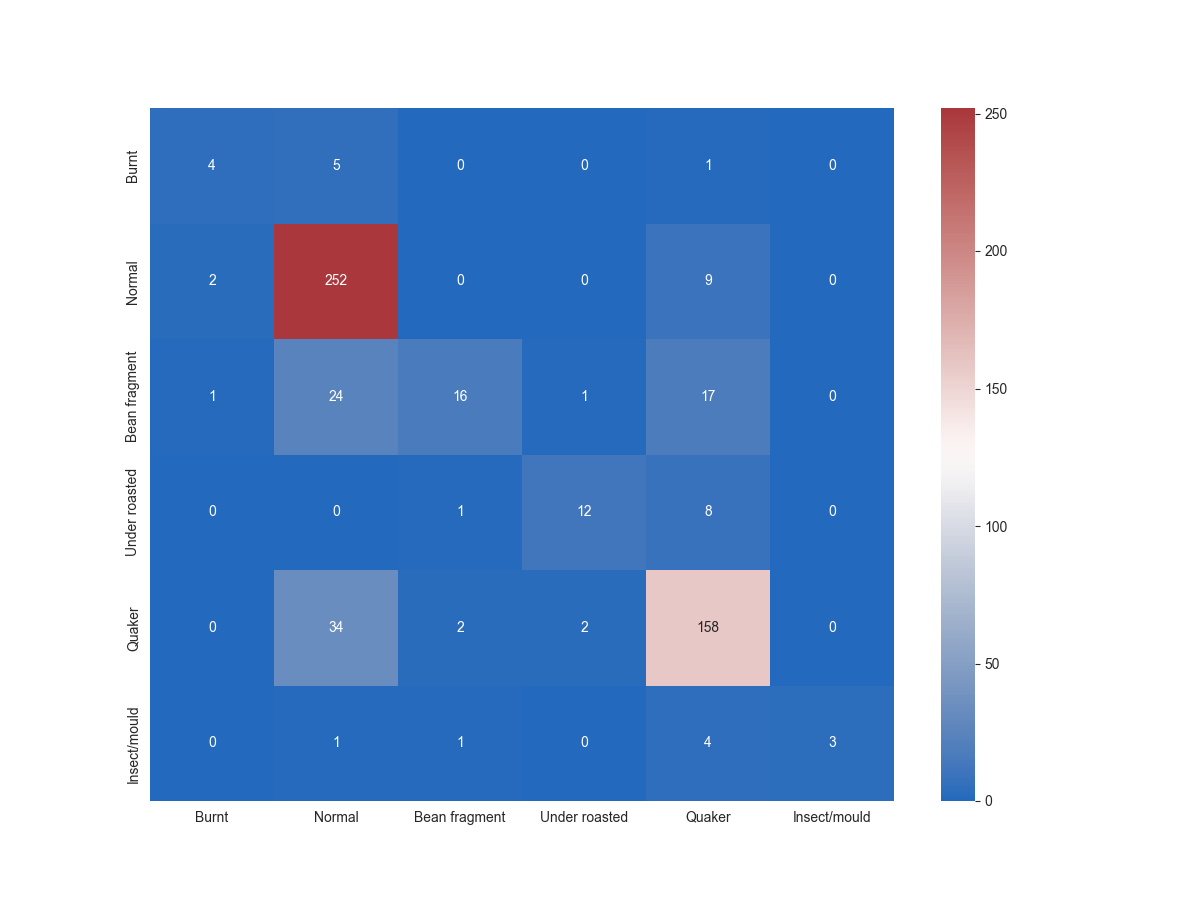
\includegraphics[width=0.8\textwidth]{figures/confusionMatrices/KNN-2}
    \caption[KNN-2]{\hyperref[tab:knnResults]{KNN-2}}
    \label{fig:knn-2}
\end{figure}

\begin{figure}[!ht]
    \centering
    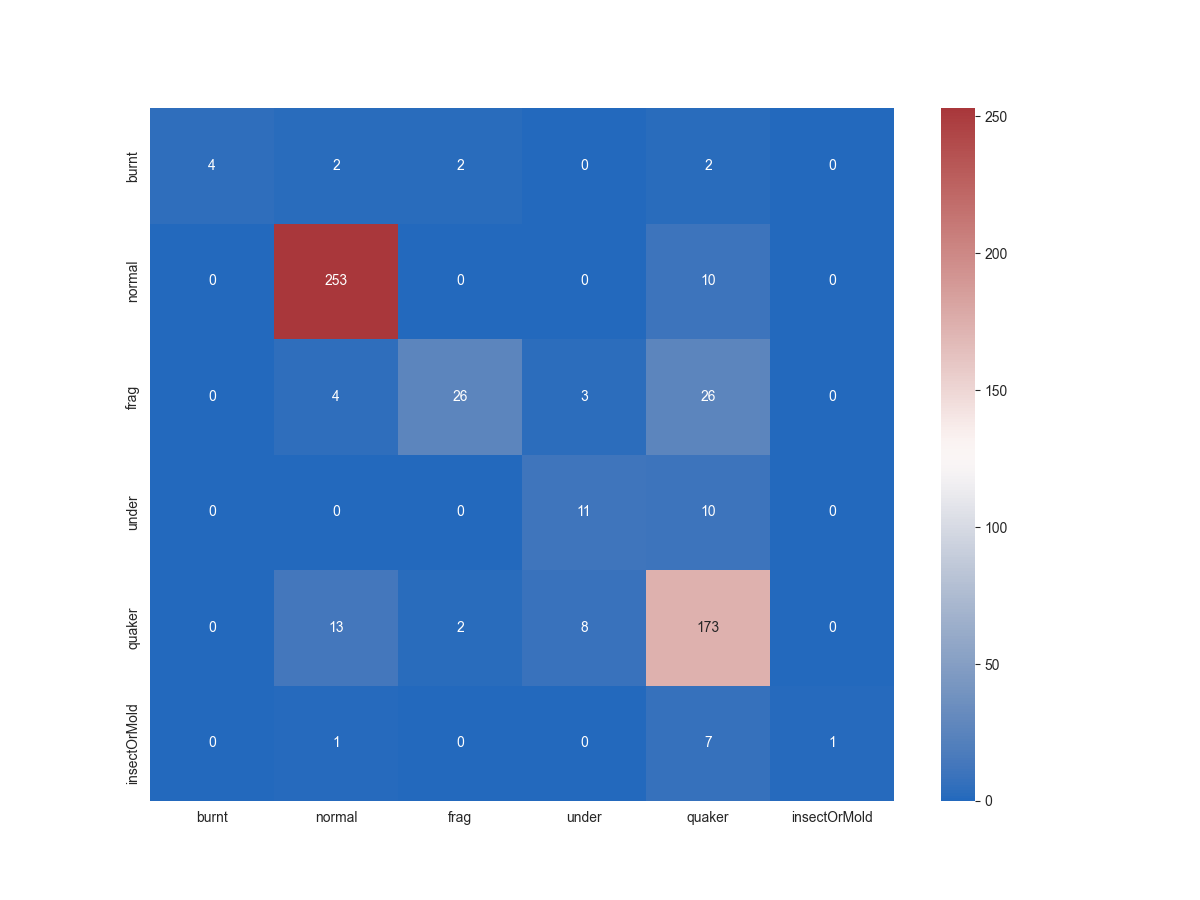
\includegraphics[width=0.8\textwidth]{figures/confusionMatrices/mobileNet-no-pretraining0-5gamma}
    \caption{MobileNet (no pre-training)}
    \label{fig:mobileNetNoPt}
\end{figure}

\begin{figure}
    \centering
    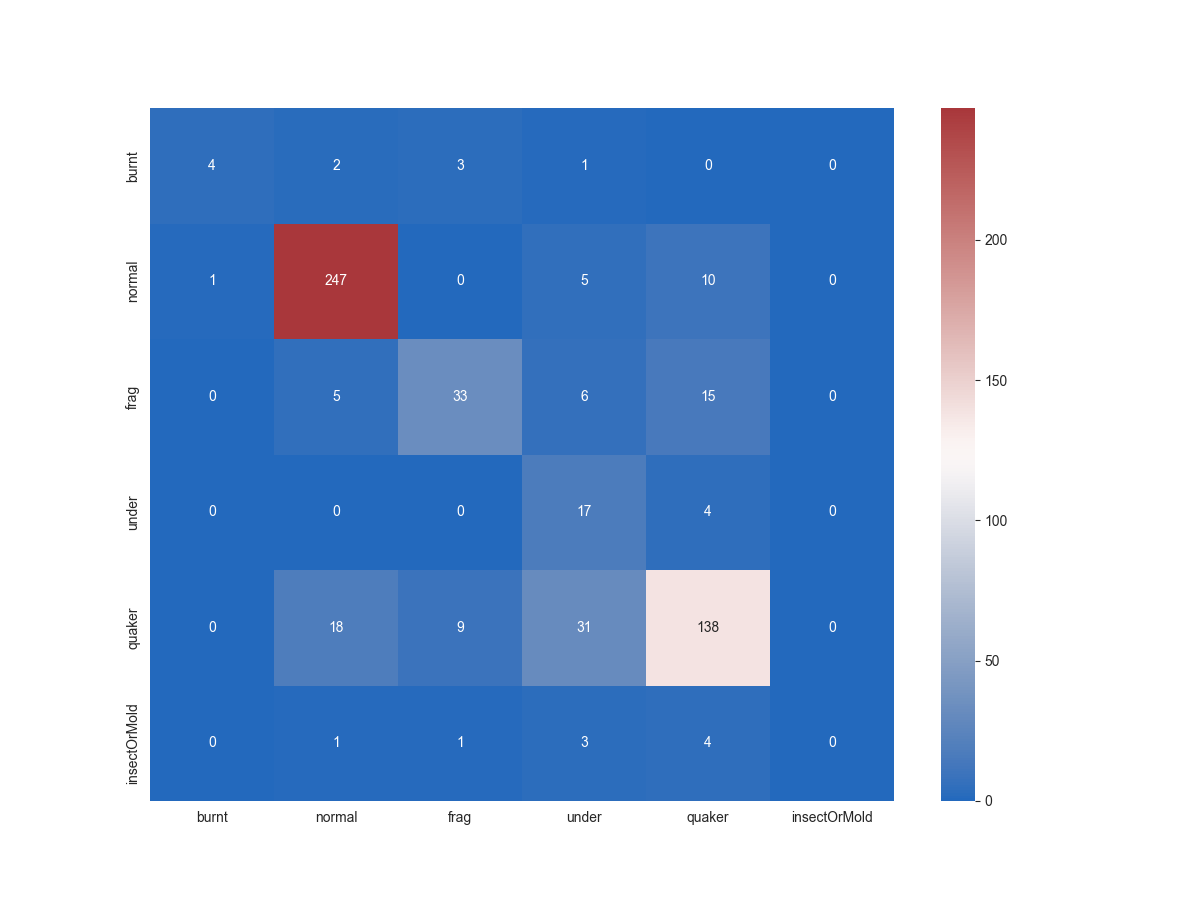
\includegraphics[width=\textwidth]{figures/confusionMatrices/shufflenet-no-pretraining0-5gamma}
    \caption{ShuffleNet (no pre-training)}
    \label{fig:shuffleNet}
\end{figure}

\begin{figure}
    \centering
    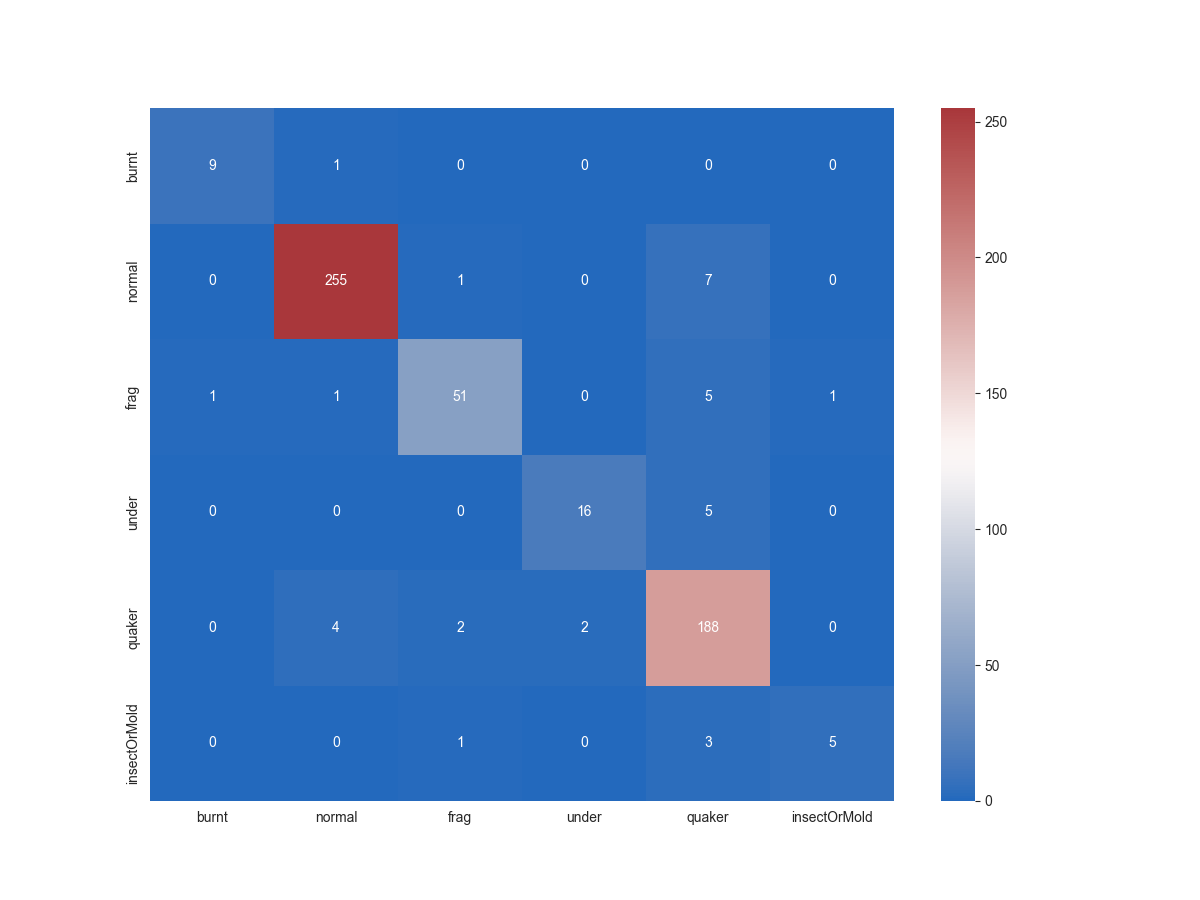
\includegraphics[width=\textwidth]{figures/confusionMatrices/resnet_18_93_acc}
    \caption{ResNet 18 (pre-trained)}
    \label{fig:resnet18}
\end{figure}

\begin{figure}
    \centering
    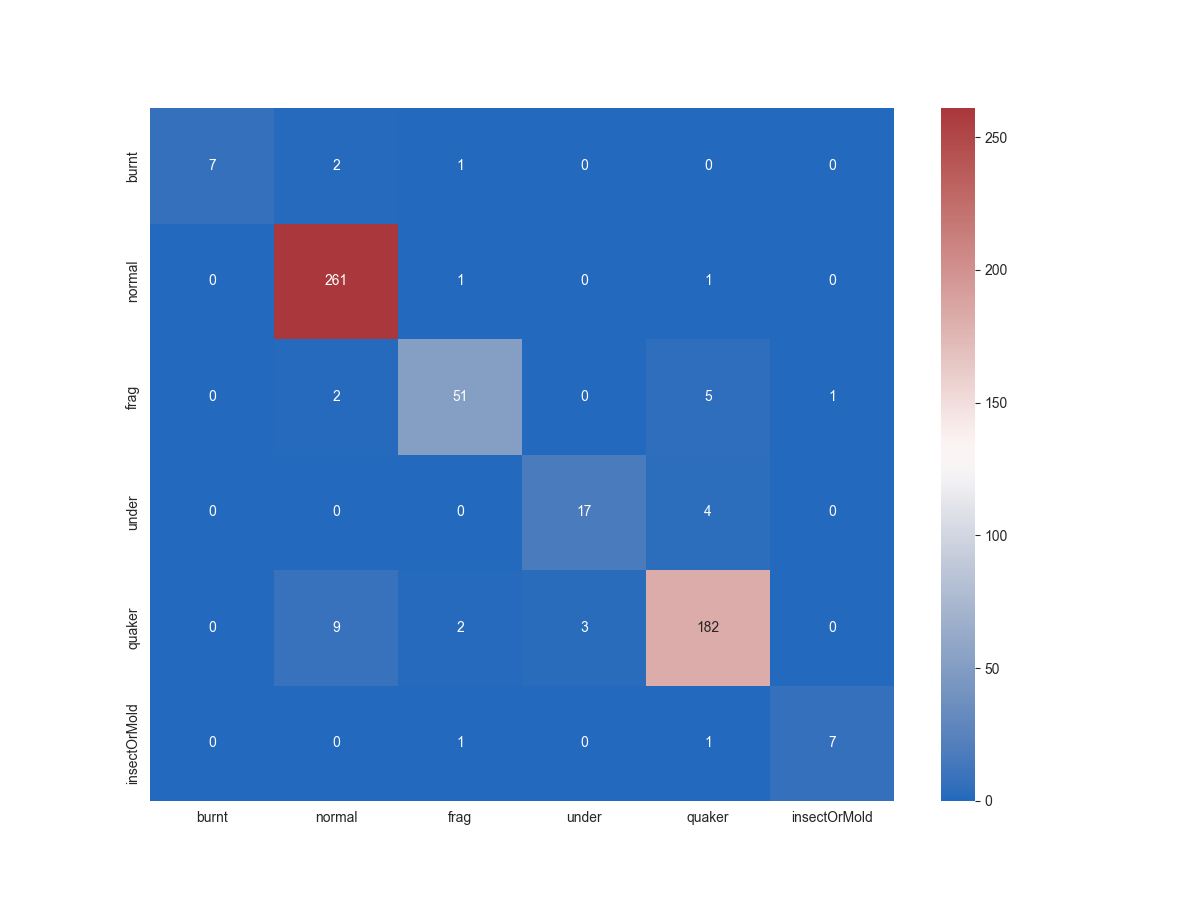
\includegraphics[width=\textwidth]{figures/confusionMatrices/resnet_34_whitebg_94_acc_8_batch}
    \caption{ResNet 34 (pre-trained)}
    \label{fig:resnet34}
\end{figure}

\begin{figure}
    \centering
    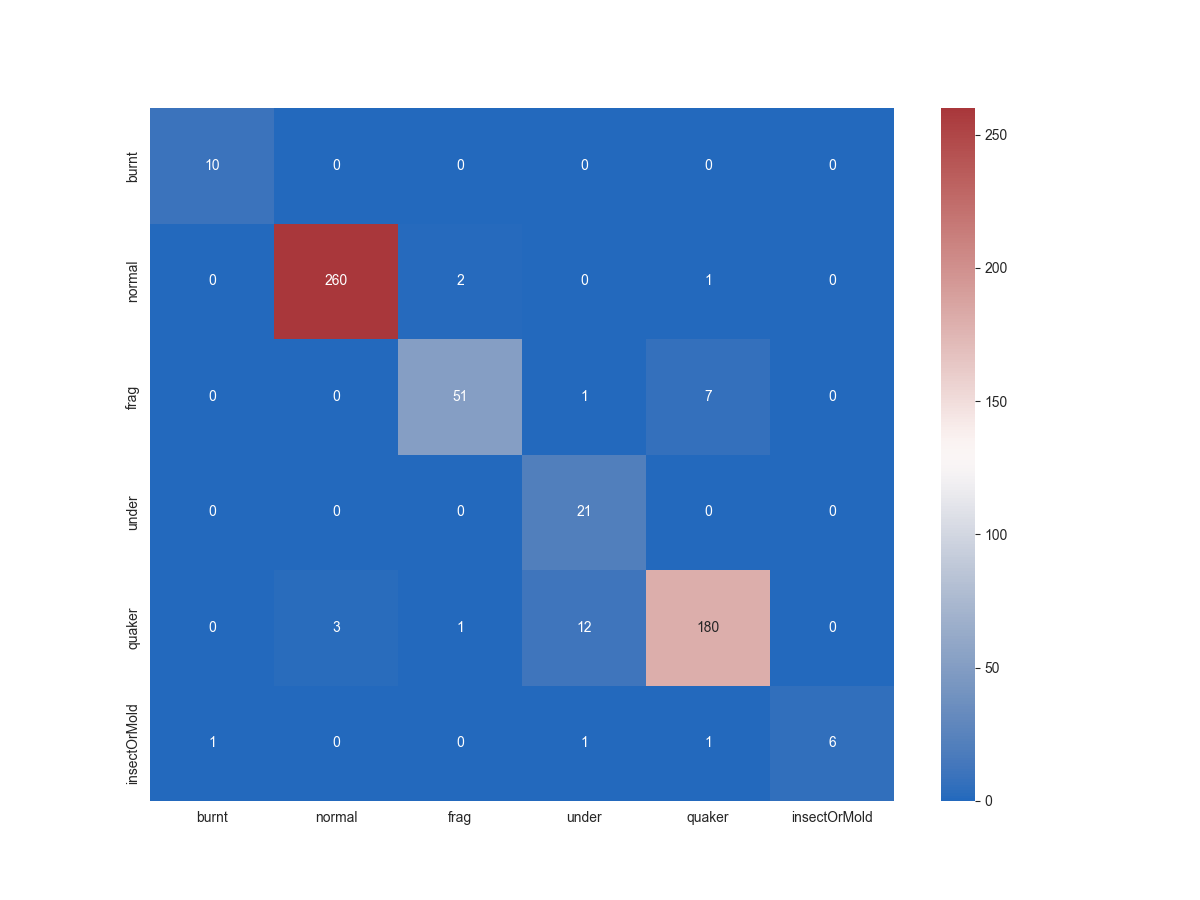
\includegraphics[width=\textwidth]{figures/confusionMatrices/resnet_50_95_acc}
    \caption{ResNet 50 (pre-trained)}
    \label{fig:resnet50}
\end{figure}

\begin{figure}
    \centering
    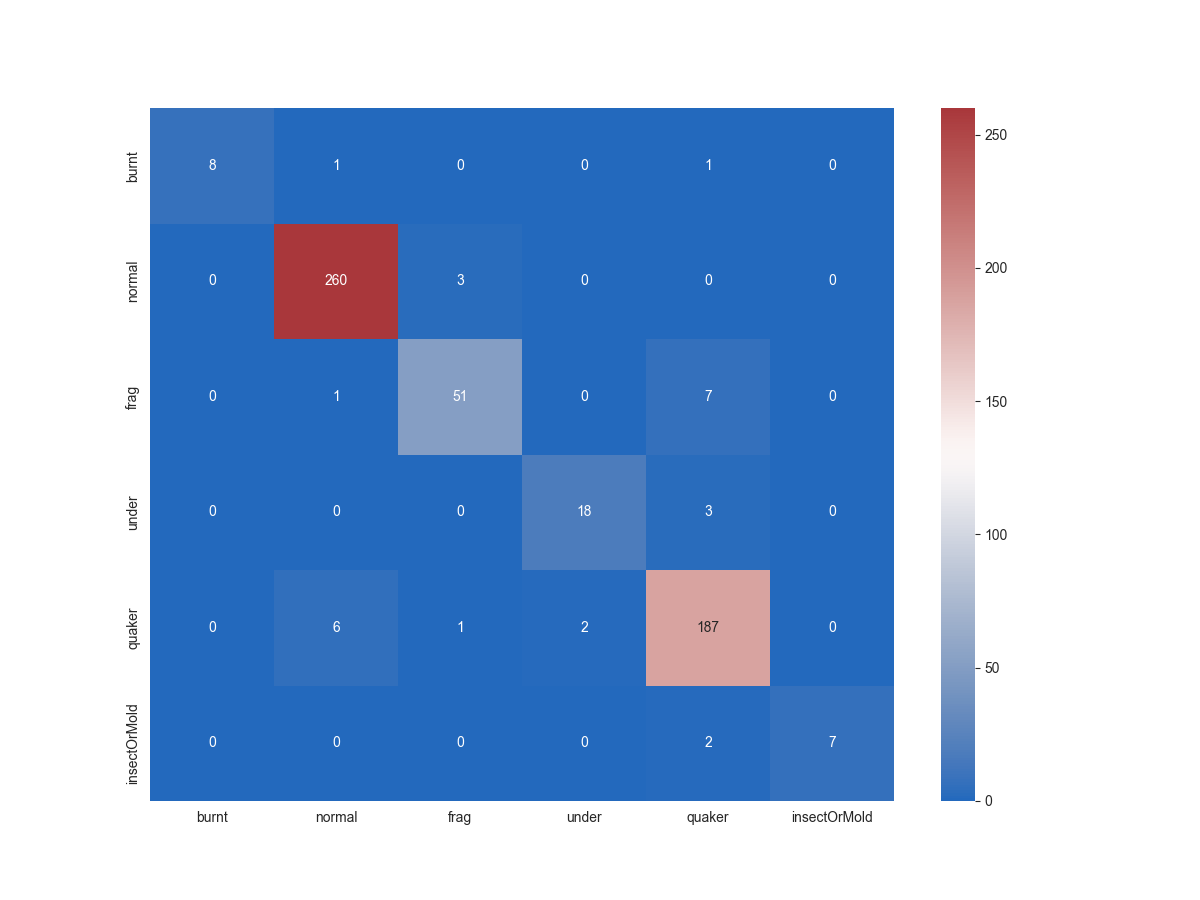
\includegraphics[width=\textwidth]{figures/confusionMatrices/mobilenet-95acc}
    \caption{MobileNet (pre-trained)}
    \label{fig:mobileNetPt}
\end{figure}

\begin{figure}
    \centering
    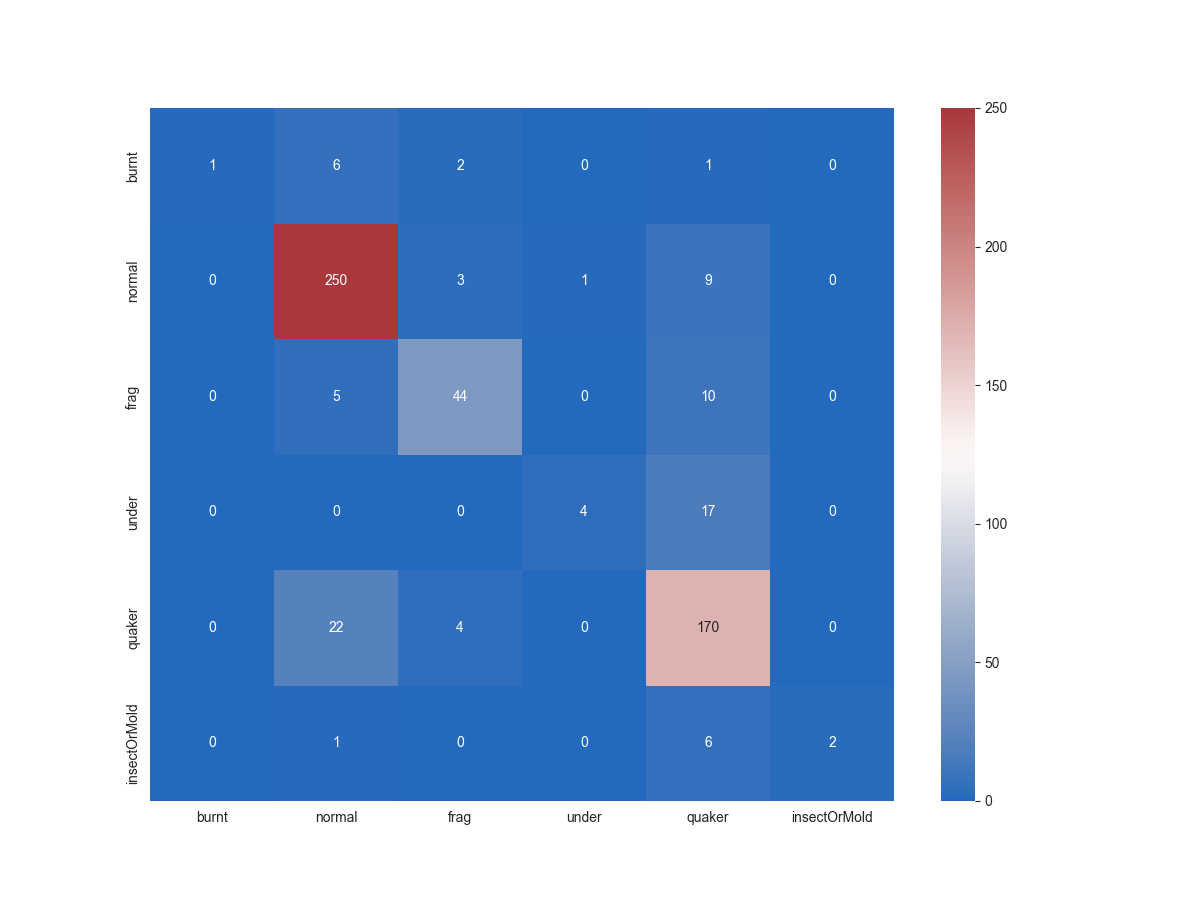
\includegraphics[width=\textwidth]{figures/confusionMatrices/swin_b_85_acc_4_batch}
    \caption{Swin transfomer (pre-trained, only last layer weights tracked)}
    \label{fig:swin}
\end{figure}
